%\chapter{Statistische Erhebung zum Spiel Æthershards}
%\label{cha:location-based_games}




%\section{Wahl des Anbieters} 
%\label{sec:}
%Evtl. auslassen\\
%Großer Zeitaufwand\\
%Viele Anbieter sind nicht kostenlos.

\section{Statistische Erhebung zum Spiel Æthershards}
%Einzelne Fragestellungen und Ergebnisse im Detail} 
%\label{sec:}
Um einen groben Überblick der User Experience des Spiels Æthershards zu bekommen wurde eine Umfrage erstellt. An Hand dieser Umfrage soll festgestellt werden welche Ideen des Prototyps weiter verfolgt und welche wieder verworfen werden sollen. An der Umfrage konnte in einem Zeitraum von vierzehn Tagen teilgenommen werden. Sie war anonym und wurde online durchgeführt. Dieses Angebot wurde von neunundachtzig Personen wahrgenommen. Ziel dieser Erhebung ist es durch gezielte geschlossene Fragen den Hintergrund der einzelnen Personen grob zu kategorisieren und ihren Geschmack bezüglich Videospielen zu skizzieren. Besonders wichtig sind hierbei die folgenden drei Unterpunkte. Der erste ist die Frage, ob sich die Spieler in Spielen eine Hintergrundgeschichte wünschen, der zweite ist, ob überhaupt der Wunsch besteht zum Spielen nach draußen zu gehen und der dritte ist, ob und in wie weit die Spieler gewillt sind Werbeeinblendungen anzuschauen oder das Spiel durch Micropayments zu finanzieren. Micropayments sind in diesem Zusammenhang kleine Zahlungen für virtuelle Gegenstände im Spiel. Für einen detaillierten Einblick in die Wünsche der Spieler werden zusätzlich offene Fragen zur Kritik an virtuellen Haustieren gestellt. \\
Im Folgenden werden die einzelnen Fragen der Umfrage genauer betrachtet und in Beziehung zueinander gesetzt.
\subsection{Alter und Freizeit} 
%\label{sec:}
Zunächst wird das Alter und die Freizeitbeschäftigungen betrachtet. Beim Alter wird der Fokus auf den Altersbereich von 16 bis 28 Jahren gelegt. Jüngere Personen wurden nicht befragt, ältere wurden in einem Umfragepunkt zusammengefasst. Die Freizeitbeschäftigungen sind grob in drei Kategorien eingeteilt. Die erste und am meisten gewählte Kategorie beinhaltet alle Aktivitäten, die in Verbindung mit Bildschirmen stehen, wie Computerspiele spielen und Fernsehen schauen. In der nächsten Kategorie befinden sich Aktivitäten die im Freien stattfinden. Die dritte Kategorie umfasst zwei Punkte der Umfrage, die den Titel nicht nicht nutzbare Freizeit tragen kann. Dazu gehört zu einen das auf Grund der Arbeit keine Zeit für Freizeit bleibt oder das auf Grund fehlender Motivation keiner Freizeitbeschäftigung nachgegangen wird. Obwohl beide Diagramme (\textbf{Abbildung \ref{chart:alterFreizeit}}) den Eindruck erwecken, als seien die Freizeitaktivitäten stark mit dem Alter der befragten Personen verknüpft, ist dies aber nicht der Fall. So sind die beiden Personen die bei der Frage nach der Freizeit \glqq Langeweile\grqq\ angegeben haben zwischen 20 und 24 Jahren. Des Weiteren haben auch Personen im Alter von 20 Jahren auf Grund ihrer Arbeit wenig bis keine Freizeit. 

\begin{figure}[H]
    \centering
    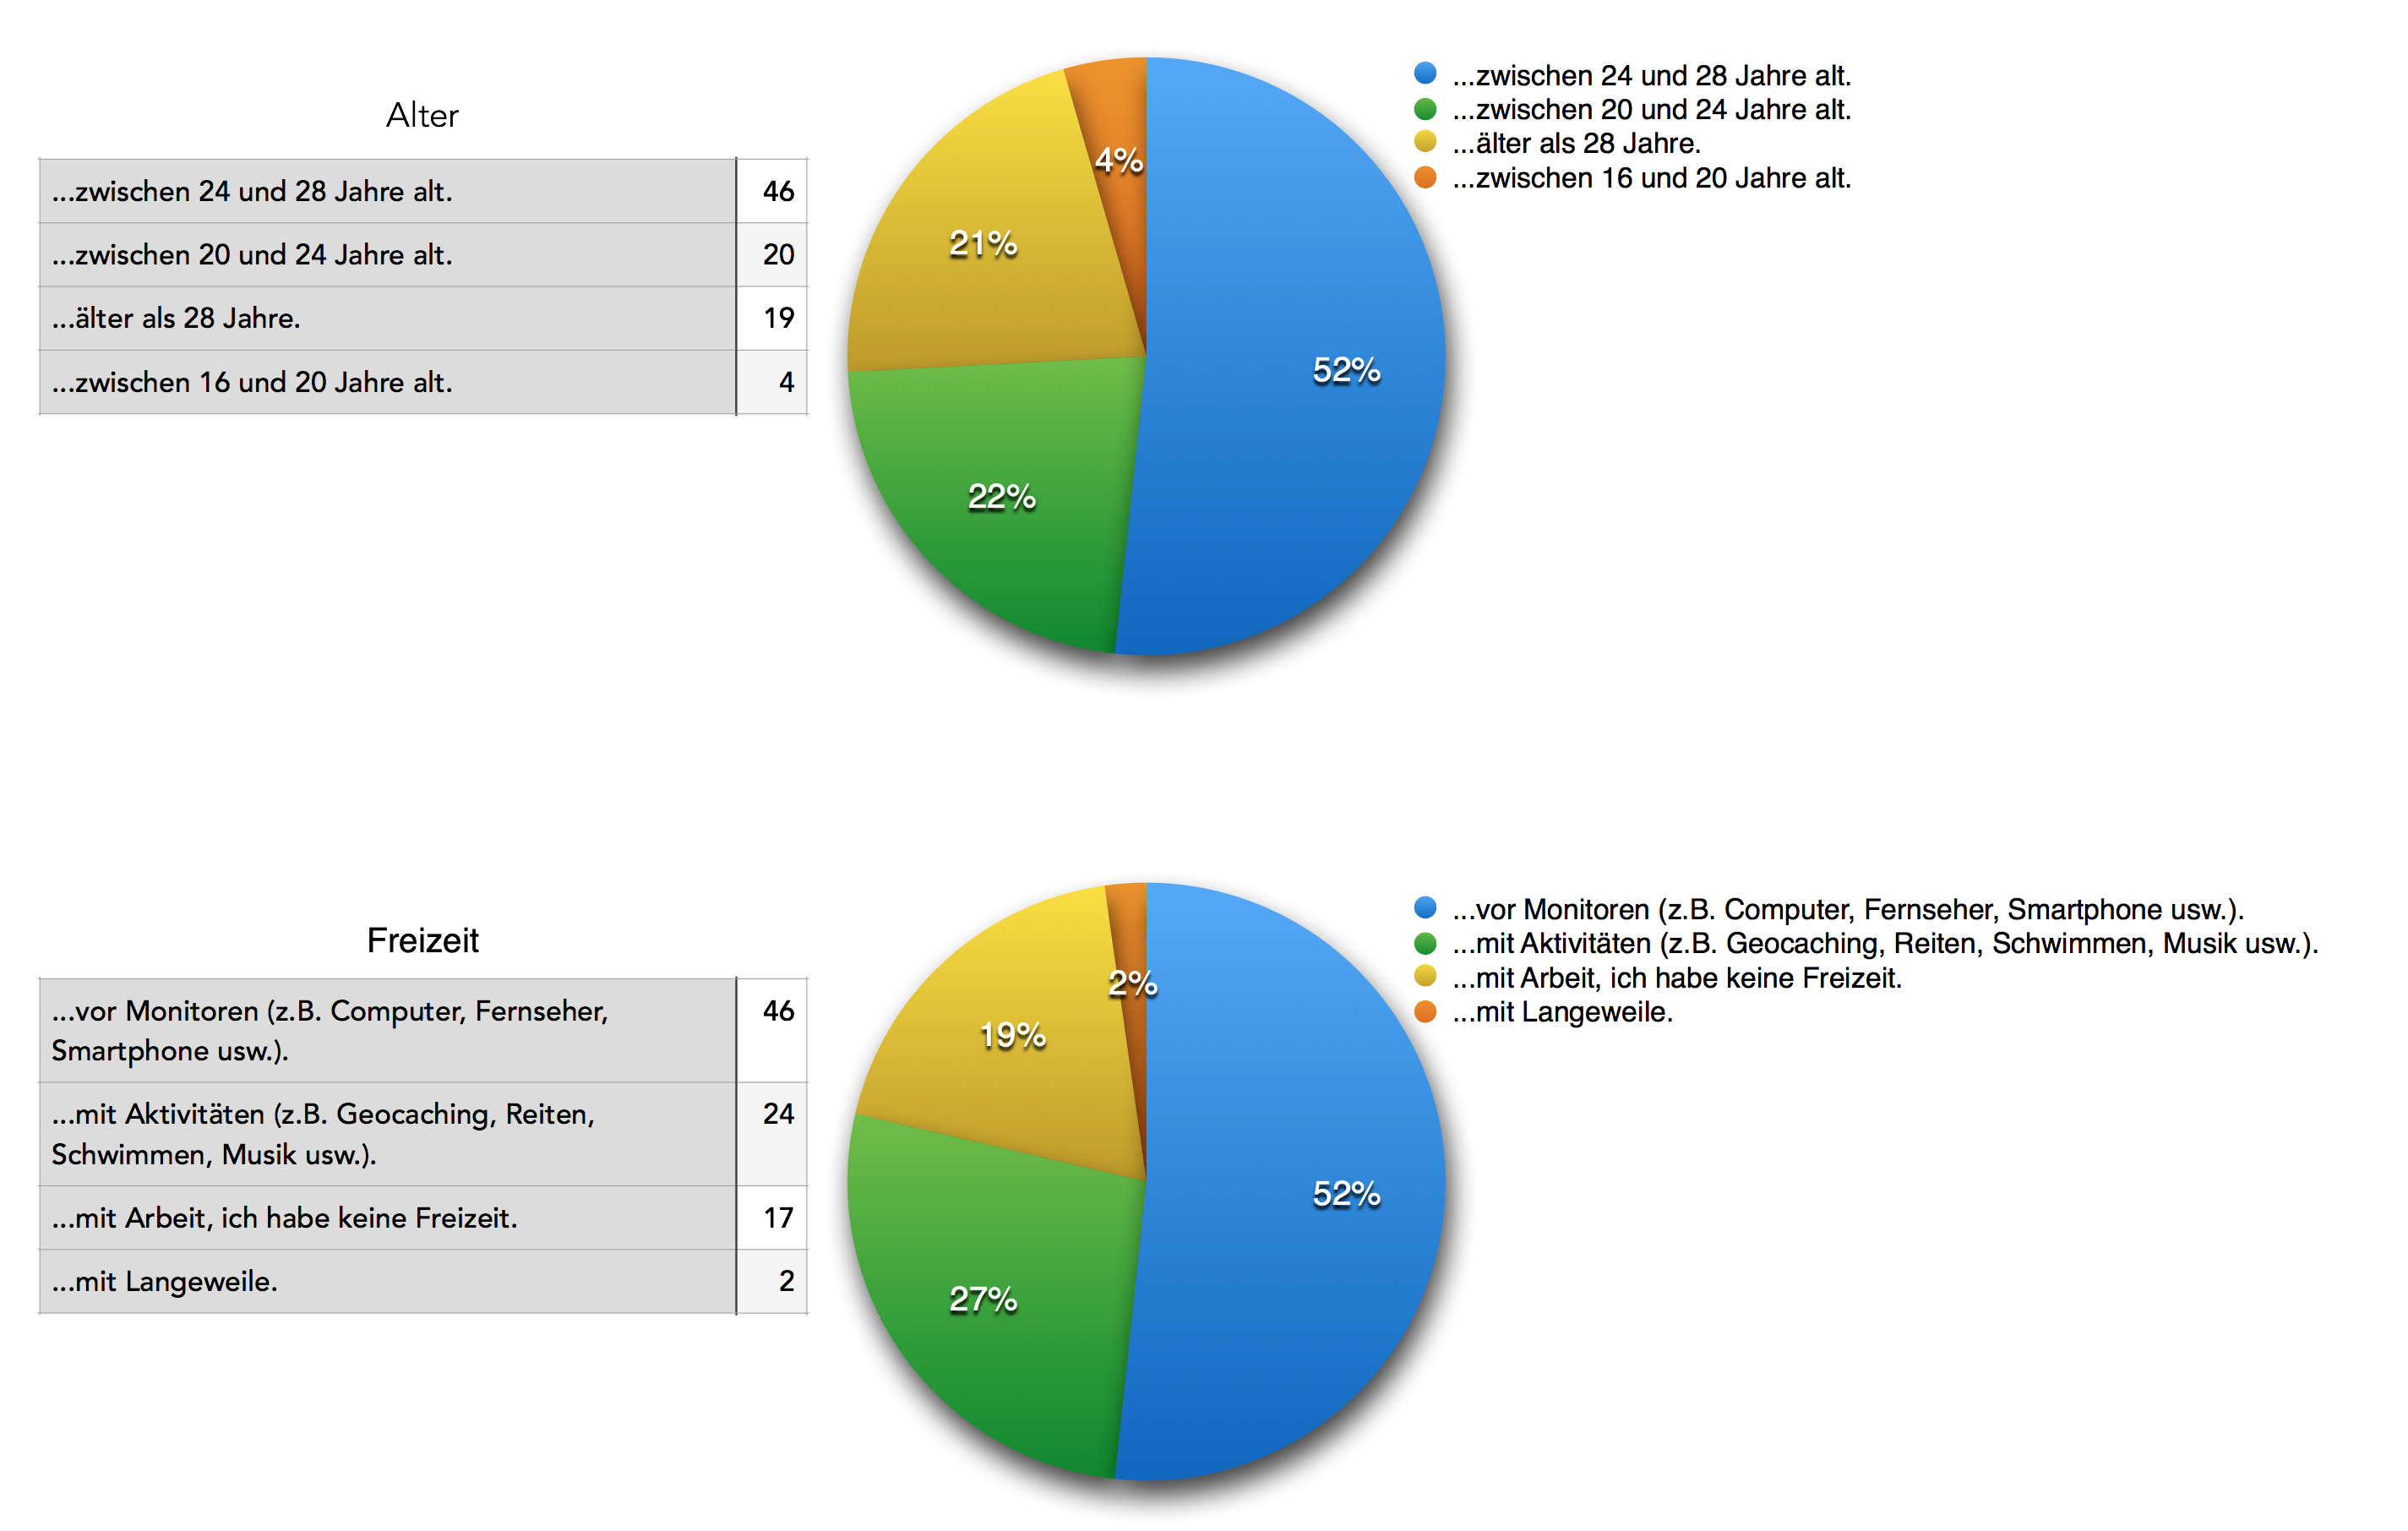
\includegraphics[width=1.01\textwidth]{files/umfrage/alterUndFreizeit}
    \caption{Alter und Freizeit}
    \label{chart:alterFreizeit}
\end{figure}


\subsection{Smartphone-Verteilung} 
%\label{sec:}

Die Fragestellung zum Smartphone soll Aufschluss darüber geben, wie sinnvoll die Entscheidung war das Spiel Plattform übergreifend zu entwickeln. Zudem bietet sich hier die Möglichkeit zum Vergleich mit einer öffentlichen Statistik, um eventuelle Abweichungen von Erhebungen größeren Umfangs festzustellen.
\begin{figure}[H]
\centering
\subfigure[Smartphone-Verteilung aus der aktuellen Umfrage]{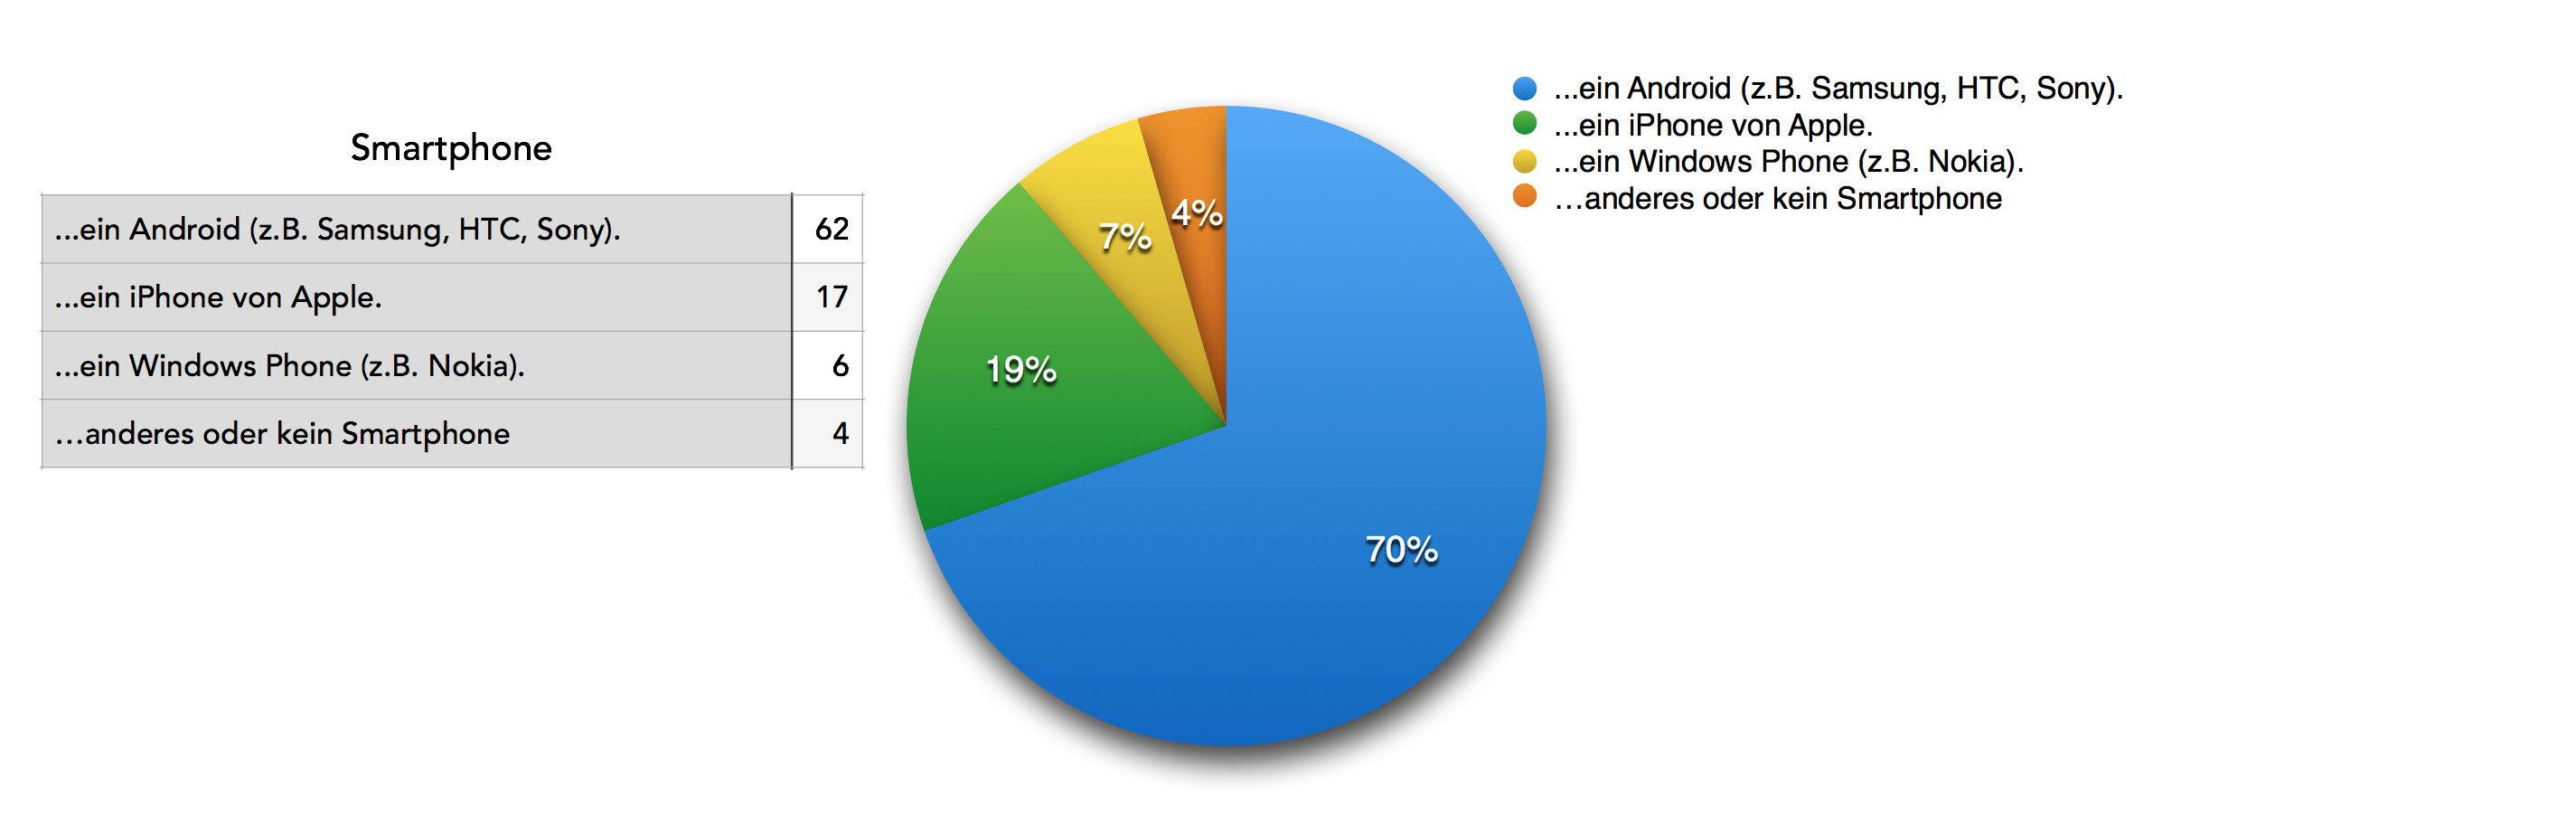
\includegraphics[width=1.01\textwidth]{files/umfrage/smartphoneVerteilungMy}}
\vfill
\subfigure[Smartphone-Verteilung nach Statista Sept. 2013 (Anzahl Befragter in Mio.) \cite{Smartphone:-KU40Zfi}] 
{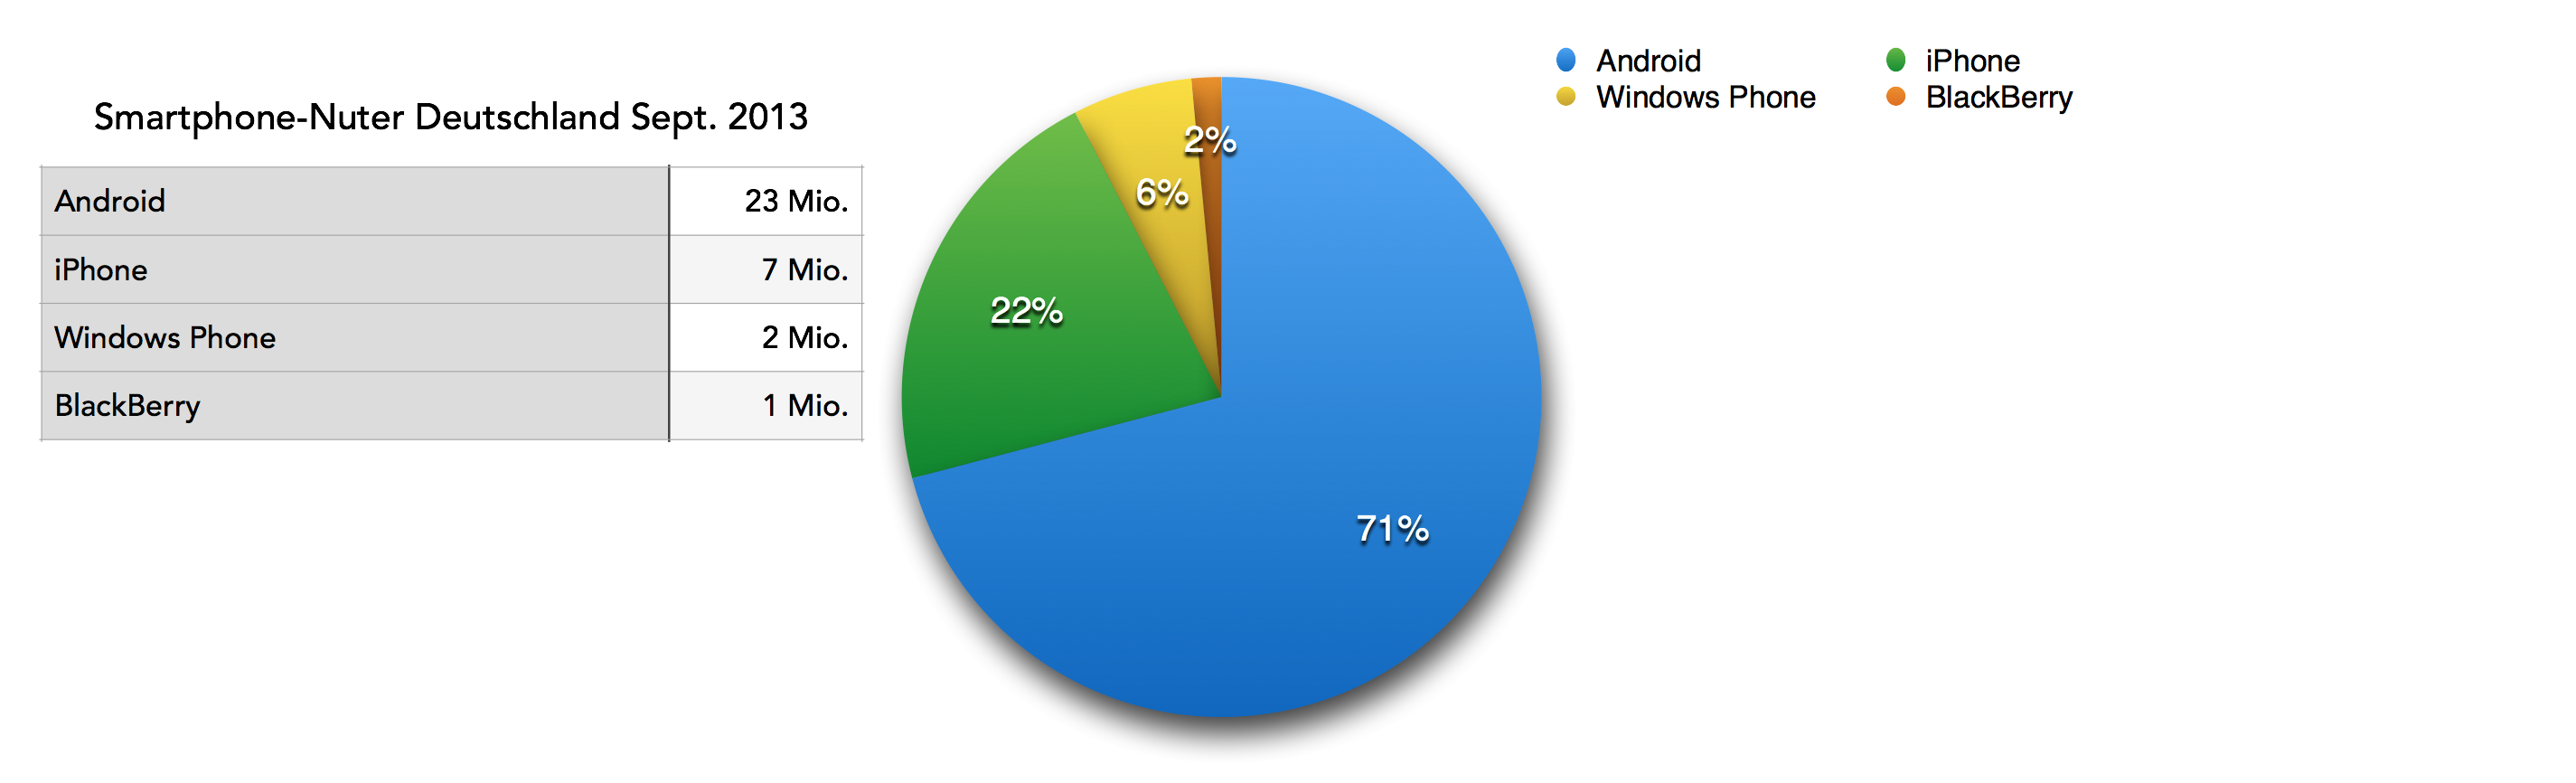
\includegraphics[width=1.01\textwidth]{files/umfrage/smartphoneVerteilungStat}}
\caption{Öffentliche und private Erhebung zur Smartphone-Verteilung}
\label{chart:smartphone}
\end{figure}

Die Verteilung in beiden Diagrammen (\textbf{Abbildung \ref{chart:smartphone}}) ist ähnlich. 
Von den Befragten besitzen ca. 70\% ein Google Android, ca. 20\% ein iPhone von Apple und ca. 7\% ein Windows Phone. Im letzten Punkt unterscheiden sich beide Erhebungen minimal. In der öffentlichen Statistik wird an dieser Stelle das BlackBerry angeführt. In der Umfrage des Authors ist dieser Punkt größer abgesteckt. So fallen hierunter weitere Smartphones sowie das Nichtvorhandensein eines Smartphones. \\
Da beide Auswertungen so nah bei einander liegen, kann davon ausgegangen werden, dass bei der vom Author gestellten Erhebung ein relevanter Querschnitt entstanden ist.\\


\subsection{Hintergrundgeschichte} 
%\label{sec:}
In der ursprünglichen Konzeption des Spieles Æthershards wurde eine Hintergrundgeschichte vorgesehen die sich episodisch zusammensetzt, so dass im Laufe der Zeit eine sehr dichte Storyline um das Spiel entstehen kann. In der Umfrage wird dies mit einer direkten Frage zur Komplexität der von Geschichten in Spielen aufgegriffen. Exakt 85\% der Befragten finden eine Hintergrundgeschichte umso besser, je detaillierter sie ist bzw. sehr gut. Weitere 12\% haben nichts gegen eine Geschichte einzuwenden, solange diese kurz gehalten wird. Lediglich 2\% der Befragten sprechen sich gegen eine Story aus. \\
Hieraus lässt sich sehr deutlich erkennen, wie wichtig eine Hintergrundgeschichte für das fertige Spiel ist und das für die Entwicklung dieser Geschichte evtl. noch zusätzliche Zeit investiert werden sollte.

\begin{figure}[H]
    \centering
    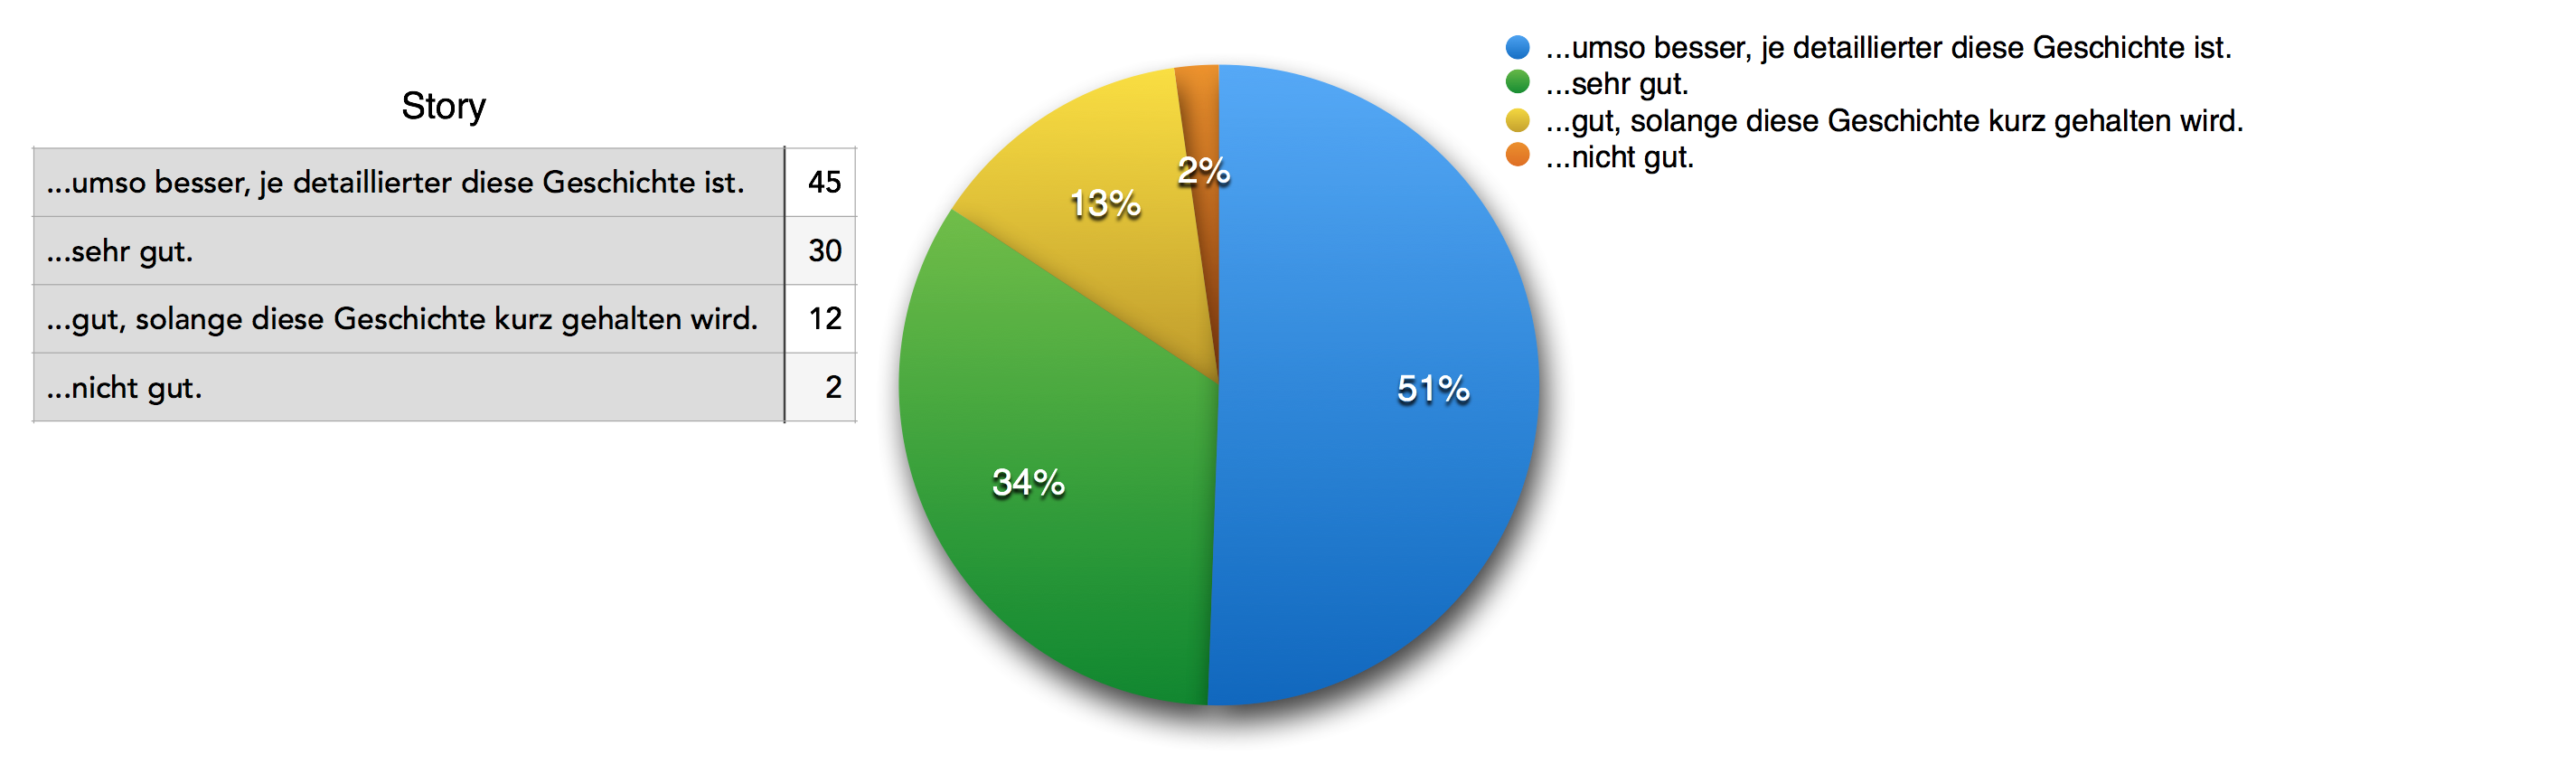
\includegraphics[width=1.01\textwidth]{files/umfrage/story}
    \caption{Antworten zu den offenen Fragen}
    %\label{chart:alterFreizeit}
\end{figure}

\subsection{Zeitlicher Rahmen und Realismus des Spiels} 
%\label{sec:}
Der zeitliche Rahmen so wie der Realismus von Æthershards ist im Vorfeld nicht klar definiert worden. In der Planung ist es darauf hinaus gelaufen, dass es in der Gegenwart spielt und sich an realistischen Elementen bedient, aber keineswegs Wert auf Realismus legt. Die Frage nach der zeitlichen Orientierung des Spiels ist daher wichtig. Aus der Umfrage ergibt sich jedoch ein sehr gemischtes Bild. So liegen die zeitlichen Abschnitte in der Beliebtheit nah beisammen. Der Großteil der Befragen hat angegeben, dass sie sich wünschen würden, das die Zeiten miteinander vermischt werden. Wie dies genau geschehen könnte wird im weiteren Verlauf der Arbeit beschrieben. \\
Zum Realismus des Spiels gehört definitiv der Location-based Aspekt. So werden Spieler immer wieder mit der wirklichen Realität konfrontiert. Im Spiel selber wird lassen sich realistische Elemente, wie das Füttern erkennen. Hier hatte sich ein Großteil der Befragten gewünscht, genau 67\%, dass im Spiel mit realistischen Elementen gespielt wird. Daher muss an dieser Stelle noch einmal überlegt werden, welche Szenarios spielbar sind und in wiefern man den Realismus steuern kann. 


\begin{figure}[H]
    \centering
    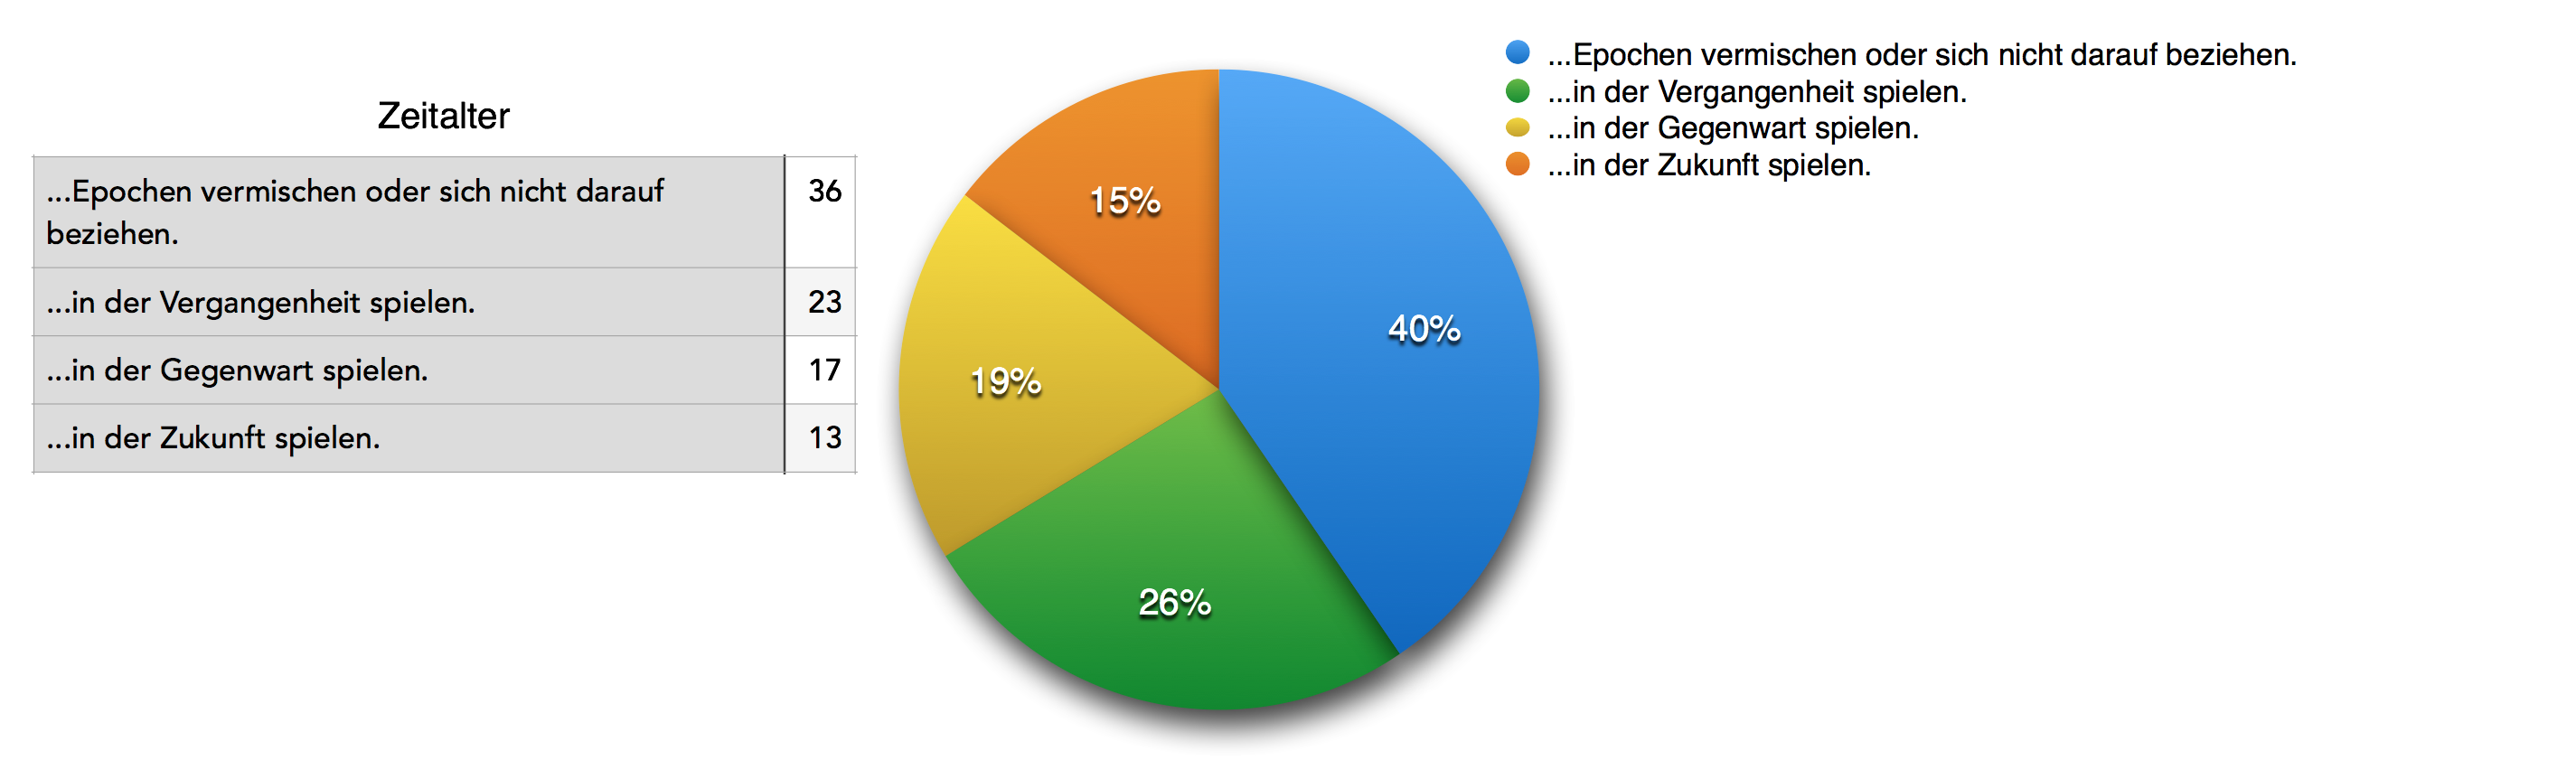
\includegraphics[width=1.01\textwidth]{files/umfrage/zeitalter}
    %\caption{Antworten zu den offenen Fragen}
    %\label{chart:alterFreizeit}
\end{figure}

\begin{figure}[H]
    \centering
    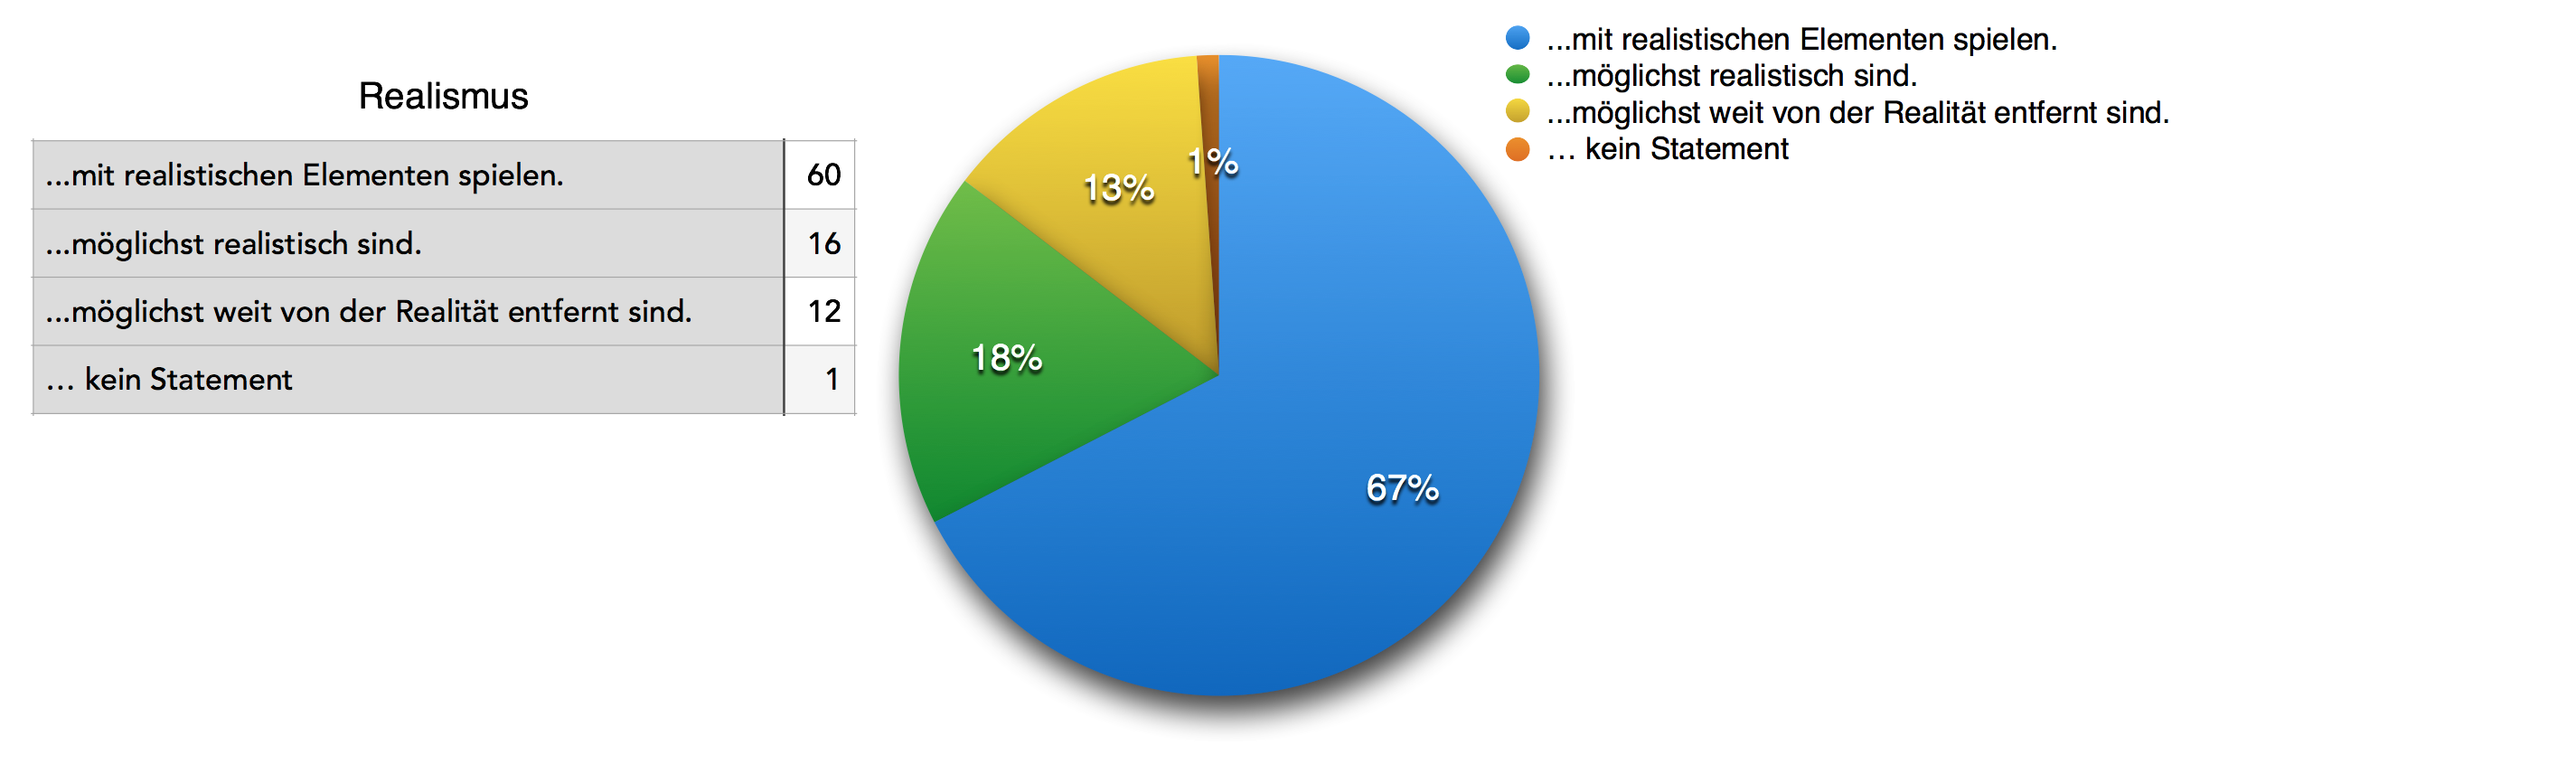
\includegraphics[width=1.01\textwidth]{files/umfrage/realismus}
    \caption{Antworten zu den offenen Fragen}
    %\label{chart:alterFreizeit}
\end{figure}


\subsection{Spielen im Freien} 
%\label{sec:}
Diese Frage soll Aufschluss darüber geben, ob potentielle Spieler überhaupt Spaß daran hätten ein Videospiel außer Haus zu spielen. Der Großteil, 81\% der Befragten, finden Idee Spiele im Freien zu spielen gut. Dies ist ein gutes Zeichen, dass die Mehrheit der Spieler auch ein Location-based Game anspielen würden. 

\begin{figure}[H]
    \centering
    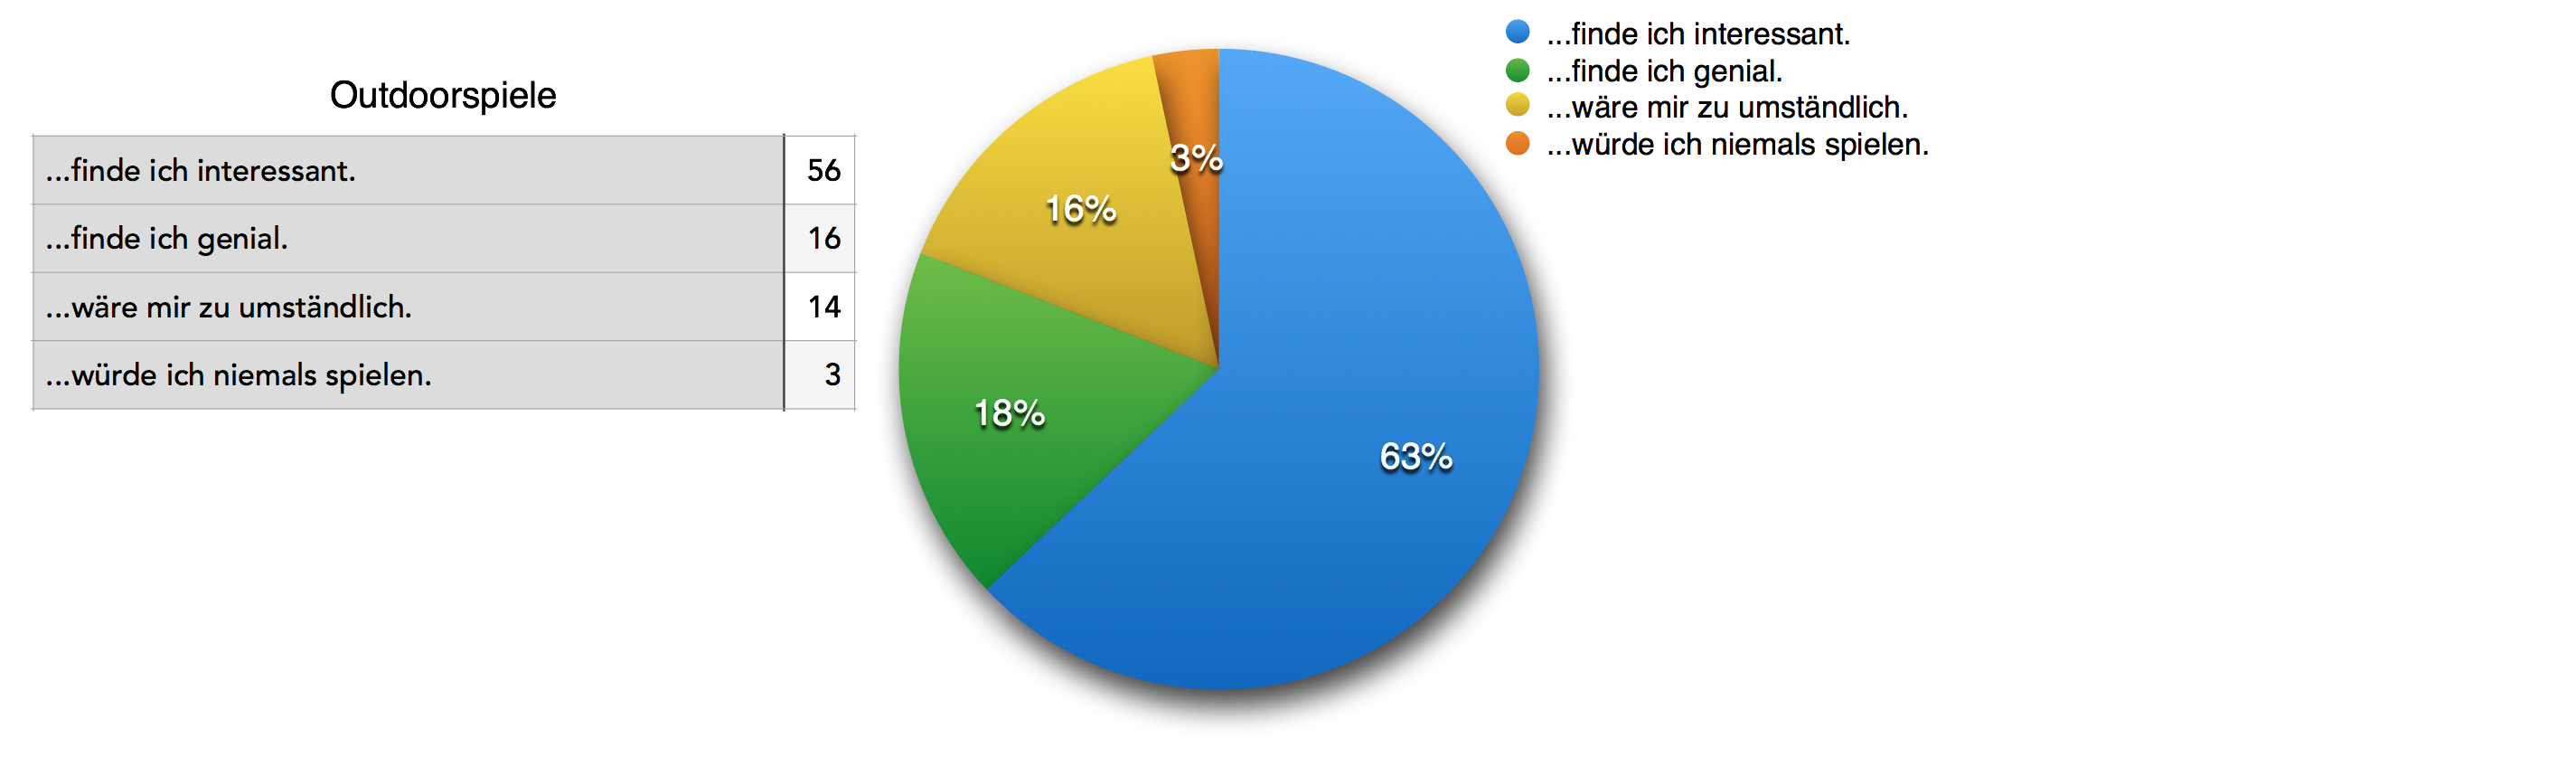
\includegraphics[width=1.01\textwidth]{files/umfrage/outdoorspiele}
    \caption{Antworten zu den offenen Fragen}
    %\label{chart:alterFreizeit}
\end{figure}


\subsection{Ertragsmöglichkeiten}
%\label{sec:}
Für eine App bieten sich verschiedene Einnahmequellen an. Die Möglichkeiten wären ein Festpreis, Werbeeinblendungen  
Keine Werbung im Spiel, eher Micropayments

Wesentlich mehr Android besitzer, aber: 

\glqq Im Klartext heißt das, wenn ein Entwickler mit einer iOS-App im App Store 1 Euro verdient, spielt die gleiche App für Android im Amazon Appstore 0,89 Euro ein und im Google Play Store nur 0,23 Euro.\grqq\

Quelle: \url{http://www.mobiflip.de/android-apps-und-ihre-einnahmen-amazon-appstore-knapp-hinter-apple-app-store-google-play-abgeschlagen/}

\begin{figure}[H]
    \centering
    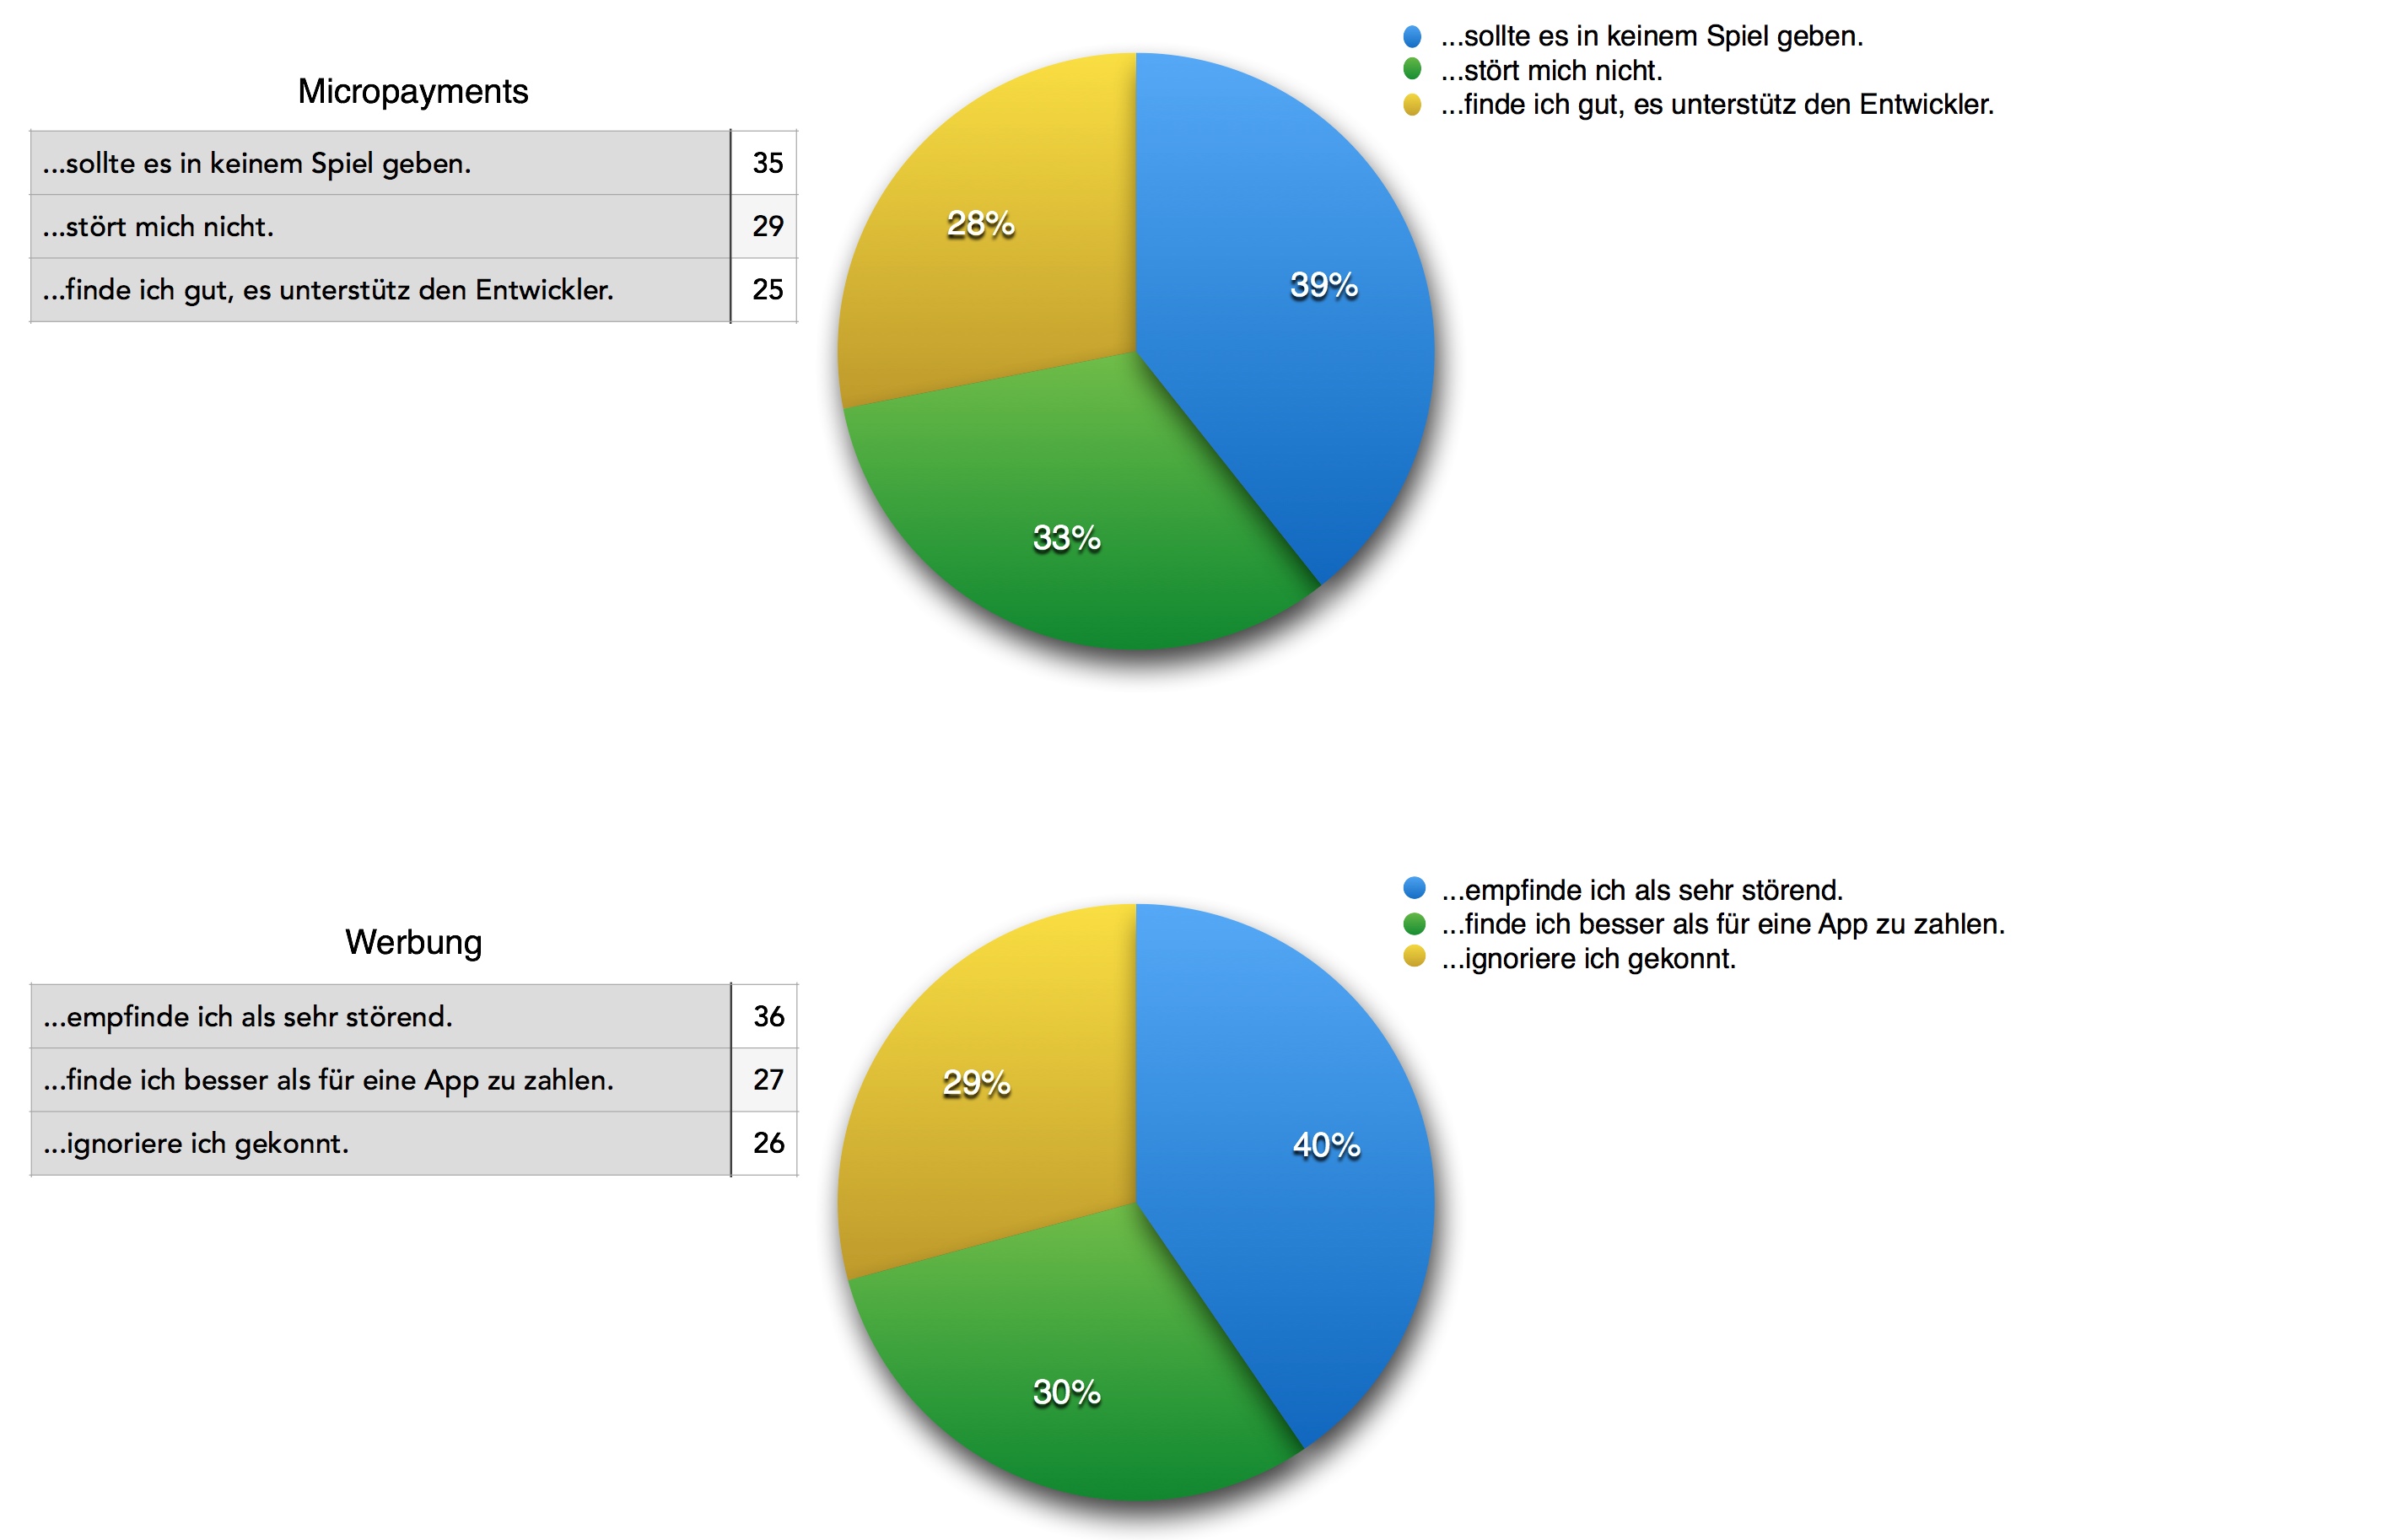
\includegraphics[width=1.01\textwidth]{files/umfrage/finanzierung}
    \caption{Antworten zu den offenen Fragen}
    %\label{chart:alterFreizeit}
\end{figure}



\subsection{Kritik an virtuellen Haustieren}
%\label{sec:}

\begin{figure}[H]
    \centering
    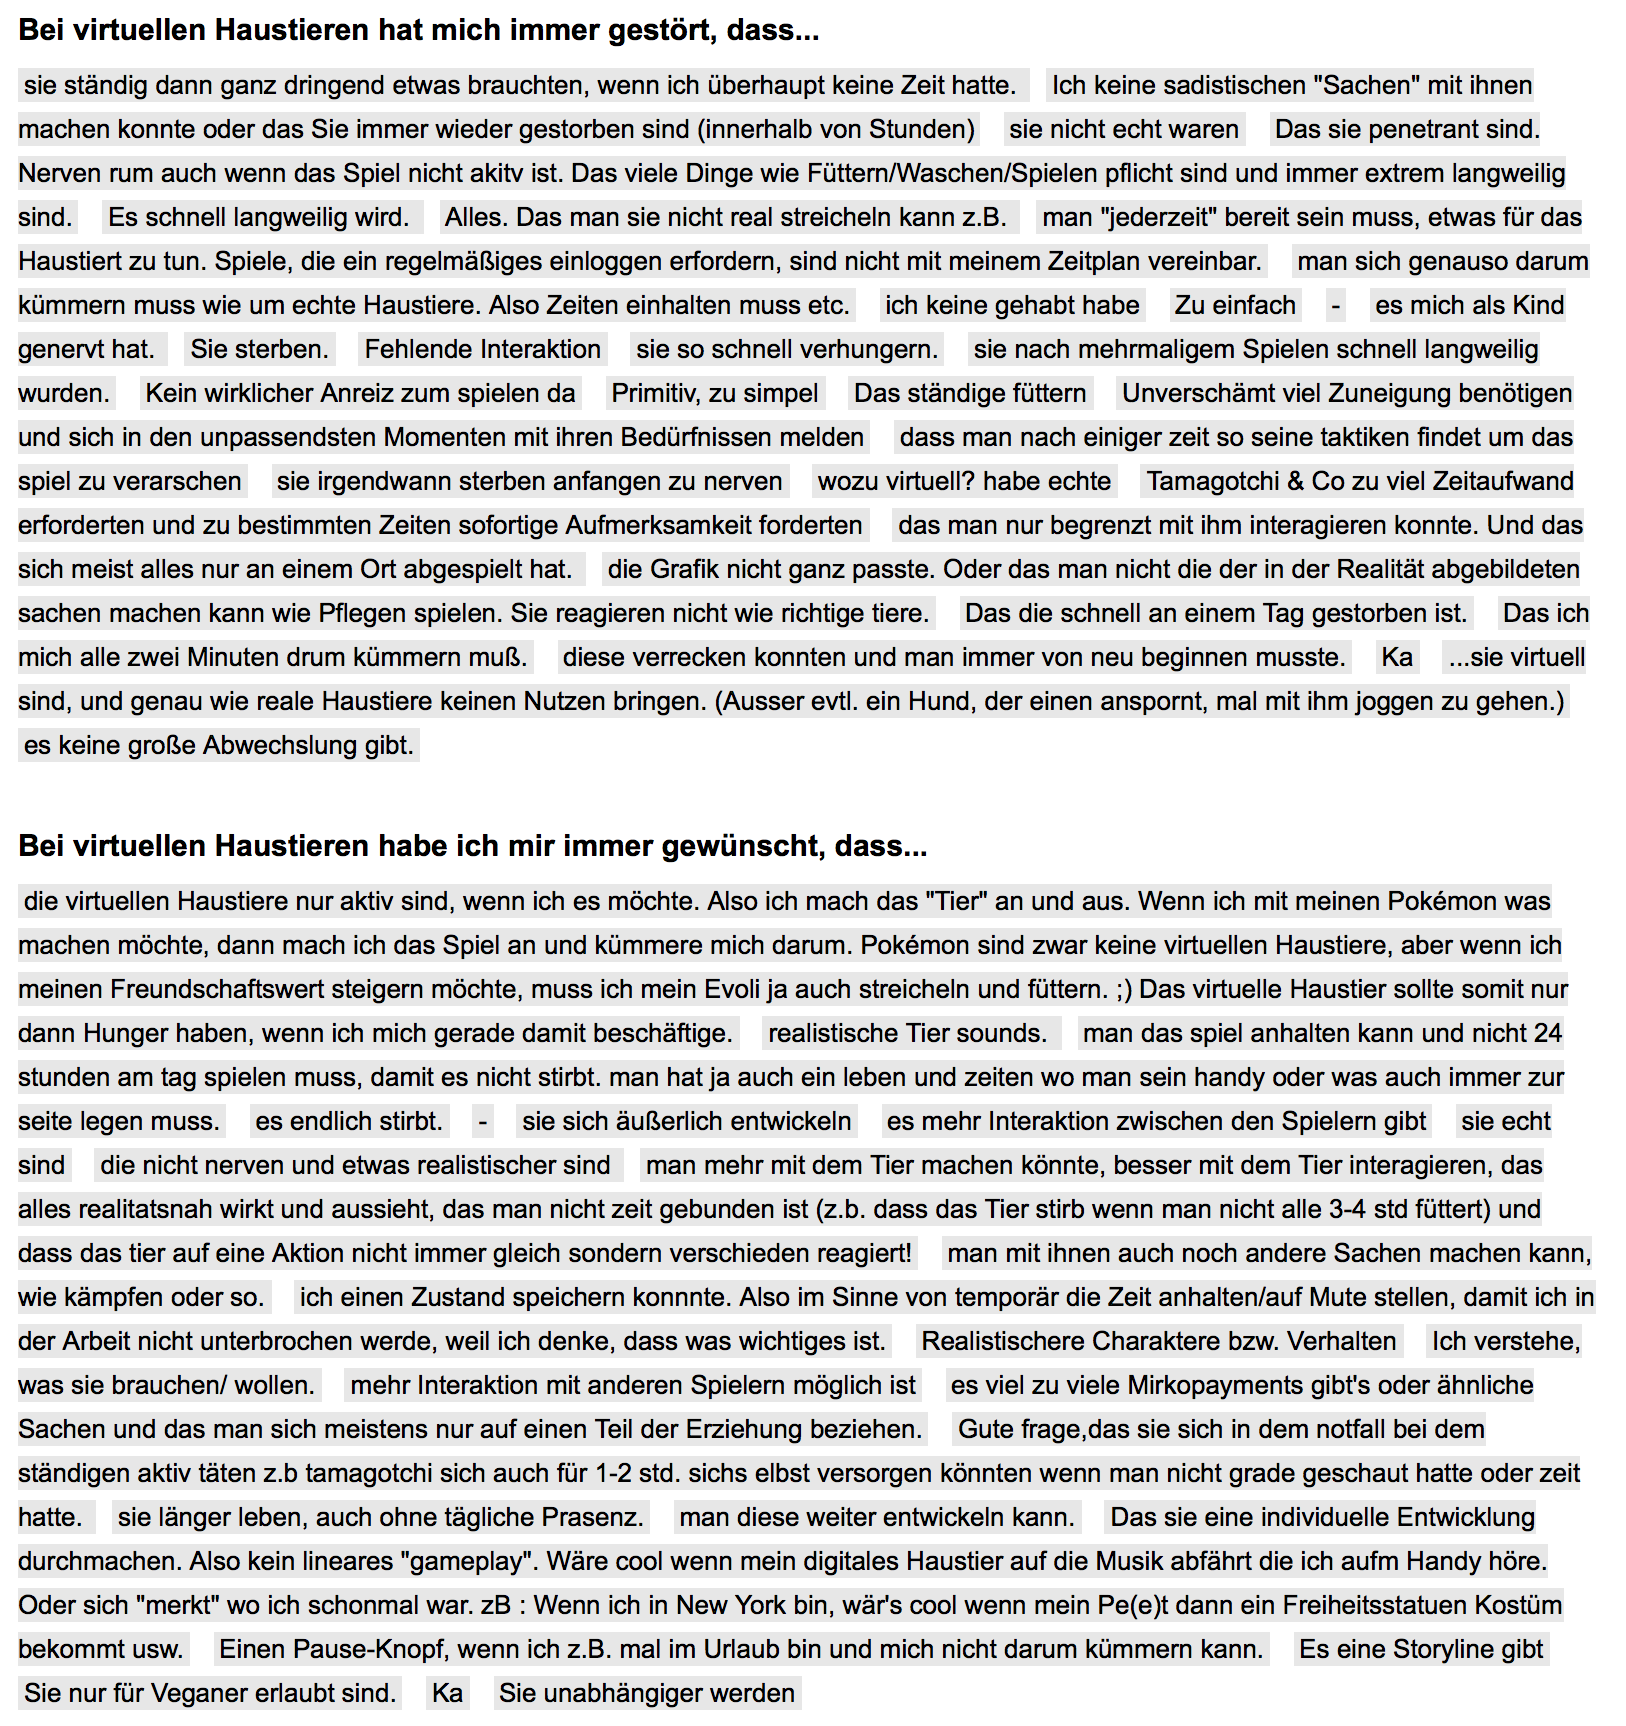
\includegraphics[width=1.01\textwidth]{files/umfrage/einzelErgebnisse}
    \caption{Antworten zu den offenen Fragen}
    %\label{chart:alterFreizeit}
\end{figure}

Zu zeitintensiv, störend, zu viel Aufmerksamkeit benötigt, sterben zu schnell, schnell langweilig, zu wenig Interaktionsmöglichkeiten, zu simpel, keinen nutzen, keine abwechslung, mehr realismus, mehr oder überhaupt Entwicklungsstufen, Storyline 

Micropayments auf vorhriges Kapitel beziehen (oft zu viele im Spiel).


\section{Erkenntnisse basierend auf der statistischen Erhebung} 
%\label{sec:}

